\documentclass[spanish]{beamer}
%\documentclass[compress]{beamer} % si queremos los marcos más pequeños
%
%%%%%%%%%%%%%%%%%%%%%%
% Podemos elegir como van a lucir las diapositivas.
%%%%%%%%%%%%%%%%%%%%%%
% Para mas temas, colores y fuentes ver:
% http://deic.uab.es/~iblanes/beamer_gallery/index_by_theme.html
%%%%%%%

% Temas disponibles
\usetheme{Warsaw} %%{AnnArbor} {Antibes} {Bergen} {Berkeley} {Berlin} {Boadilla} {boxes} {CambridgeUS} {Copenhagen} {Darmstadt} {default} {Dresden} {Frankfurt} {Goettingen} {Hannover} {Ilmenau} {JuanLesPins} {Luebeck} {Madrid} {Malmoe} {Marburg} {Montpellier} {PaloAlto} {Pittsburgh} {Rochester} {Singapore} {Szeged} {Warsaw}

% Paletas de colores preconfiguradas
\usecolortheme{default} %%{albatross} {beaver} {beetle} {crane} {default} {dolphin} {dove} {fly} {lily} {orchid} {rose} {seagull} {seahorse} {sidebartab} {structure} {whale} {wolverine}

% Poner un color específico en la estructura
%\usecolortheme[named=brown]{structure}
%%named=black cyan green orange violet blue darkgray lightgray purple white brown gray magenta red yellow

% Poner fuente Serif (como en el artículo) en todo el documento, 
\usefonttheme{serif}
% serif solo para fórmulas
%\usefonttheme[onlymath]{serif}
% Quitar botones para pasar diapositivas
%\setbeamertemplate{navigation symbols}{} 


% Carguemos los paquetes que vayamos a necesitar
\usepackage[T1]{fontenc} % escribe con 256 caracteres, incluye letras con
        %acentos. En el PDF podremos buscar sin problema la palabra "función". Sin esto solo usa 128 caracteres y las letras con acentos son composiciones de símbolos, en este caso no podremos encontrar la palabra "función" con el buscador del lector de PDF. 
\usepackage[utf8]{inputenc} % permite escribir con acentos, ñ y ¿¡ entre 
        %otros símbolos de nuestra lengua
\usepackage[spanish]{babel} % corta palabras respetando el silabeo y 
        %pone títulos y fechas en español (ejm. Capítulo, Sección, Referencias, etc.)
\hypersetup{colorlinks=true,linkcolor=violet,urlcolor=blue} % podemos configurar %cómo se mostrarán los hipervínculos

\usepackage{tcolorbox}

\usepackage{ragged2e} % para justificar el texto en beamer
%\usepackage{animate} % para animaciones


\title[Usando Beamer]{Detección de caras generadas por IA}
\author[Ciencia de Datos 2026]{Garcia Casas Matías Gabriel \\ Palombini Pietro}
\institute[FAMAF]{\includegraphics[scale=0.2,clip, trim=100 100 100 100]{Logo-FAMAF_UNC-color-2.jpg}} %{Facultad de Matemática, Astronomía, Física y Computación}
\date{\today} %para que aparezca la fecha de hoy

\begin{document}

\begin{frame}
  \titlepage
\end{frame}


\begin{frame}{Introducción}
StyleGAN3
\begin{itemize}
    \item Es una red generativa antagónica creada por Nvidia
    \item Permite generar imágenes muy realistas de personas
\end{itemize}

\includegraphics[scale=0.4]{02_ejemplos_imagenes.png}
\end{frame}

\begin{frame}{El dataset}
Dataset de Kaggle
\begin{itemize}
    \item $10.000$ imágenes generadas por StyleGAN3
    \item $10.000$ imágenes de caras reales tomadas de FFHQ
    \item Las imágenes son RGB de tamaño $256 \times 256$
\end{itemize}
\end{frame}

\begin{frame}{Nuestro trabajo}
El trabajo consistió en extraer una variedad de features de las imágenes y probar distintos modelos sobre distintas combinaciones de estos features, que agrupamos en los siguientes bloques:
\begin{itemize}
    \item Color
    \item Textura
    \item Gradientes HOG
    \item Frecuencia
    \item Uso directo de los píxeles
\end{itemize}
Finalmente encontramos un método que extrae features a partir de las diferencias locales entre píxeles. \\
Entrenar SVM sobre ellos nos permitió obtener los mejores resultados.
\end{frame}

\begin{frame}{Features: Color}
    Se transforma la imágen a distintos espacios de color (RGB, HSV, YCbCr).\\
    Para cada canal se calcula:
\begin{itemize}
    \item La media
    \item La desviación estándar
    \item La asimetría
    \item La curtosis
    \item Un histograma de 16 bins
\end{itemize}
    Además se calculan los percentiles 9 y 95 en escala de grises.
\end{frame}

\begin{frame}{Features: Textura}
    La textura resume cómo cambian las intensidades en vecindarios pequeños.\\
    No describe la identidad de la persona, sino patrones locales de suavidad, bordes y repetición.

    \vspace{0.25cm}
    Todas estas variables se calculan sobre la imagen en escala de grises:
    \begin{itemize}
        \item Patrones Binarios Locales (LBP)
        \item Coocurrencias de niveles de gris
        \item Bordes detectados con Sobel y Canny
        \item Entropía del histograma de intensidades
    \end{itemize}

    En total, este bloque produce 187 variables por imagen.
\end{frame}

\begin{frame}{Features: Textura -- LBP}
    \begin{columns}[T,totalwidth=\textwidth]
        \begin{column}{0.47\textwidth}
            \centering
            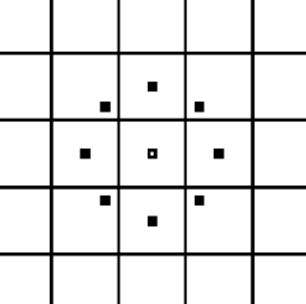
\includegraphics[width=0.72\linewidth]{lbp.png}
        \end{column}
        \begin{column}{0.50\textwidth}
            \small
            Patrones Binarios Locales (LBP) codifica cada píxel mirando sus 8 vecinos.
            \begin{itemize}
                \item Si el vecino es mayor o igual al centro, se anota 1.
                \item Si es menor, se anota 0.
                \item El patrón de ceros y unos se convierte en un código.
                \item Un histograma cuenta cuántas veces aparece cada código: cada barra corresponde a un tipo de patrón.
            \end{itemize}
        \end{column}
    \end{columns}
\end{frame}

\begin{frame}{Features: Textura -- grilla local}
    \centering
    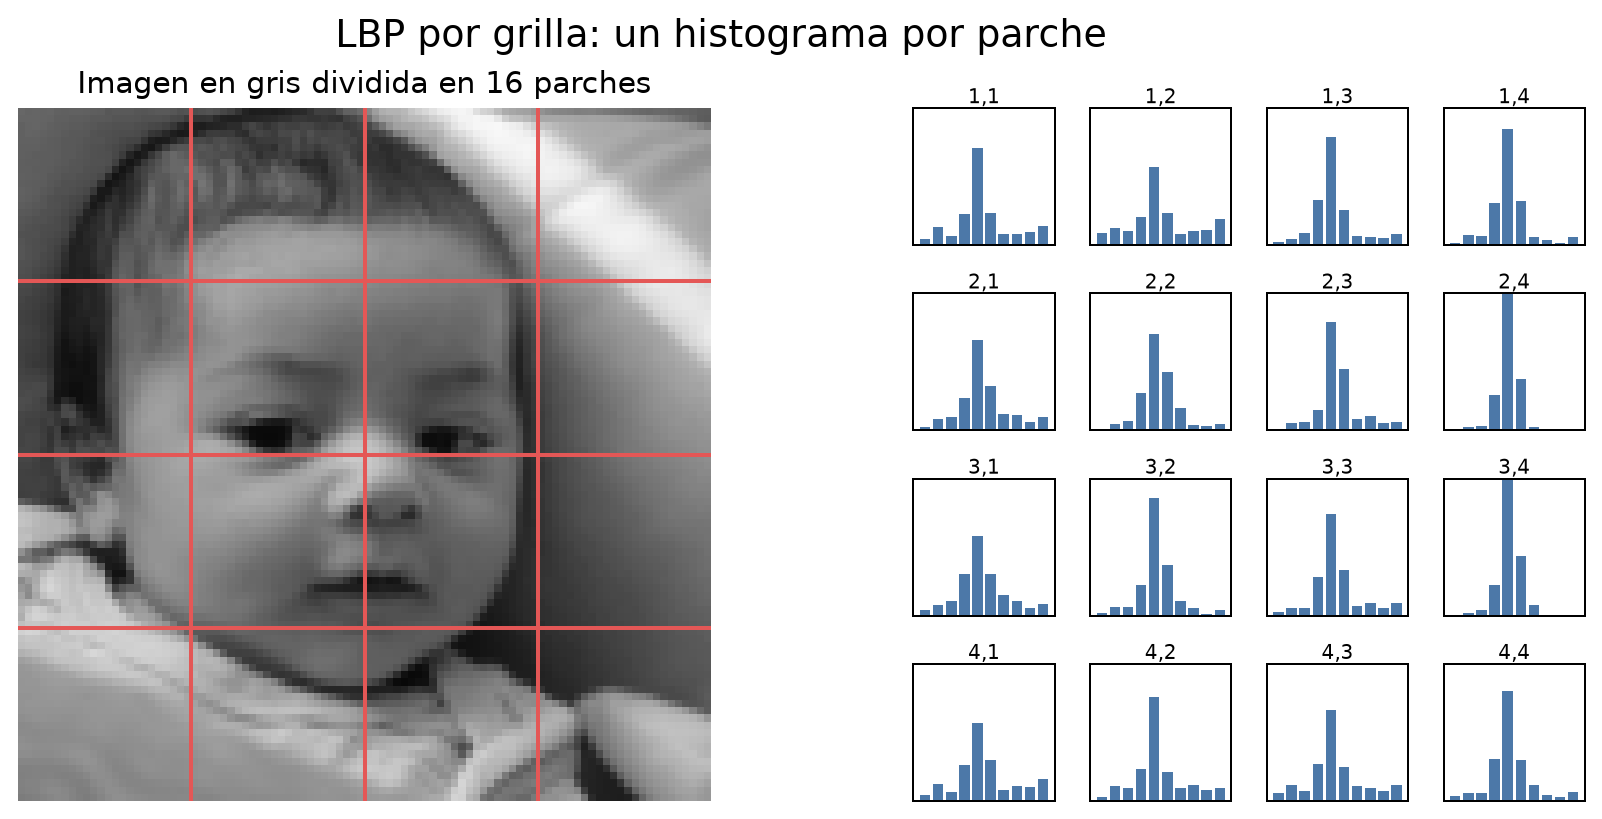
\includegraphics[width=0.95\linewidth]{texture_lbp_grid.png}

    \vspace{0.1cm}
    \small
    Además del histograma global, dividimos la imagen en una grilla $4 \times 4$ y calculamos un histograma LBP en cada parche.
\end{frame}

\begin{frame}{Features: Textura -- coocurrencias}
    \centering
    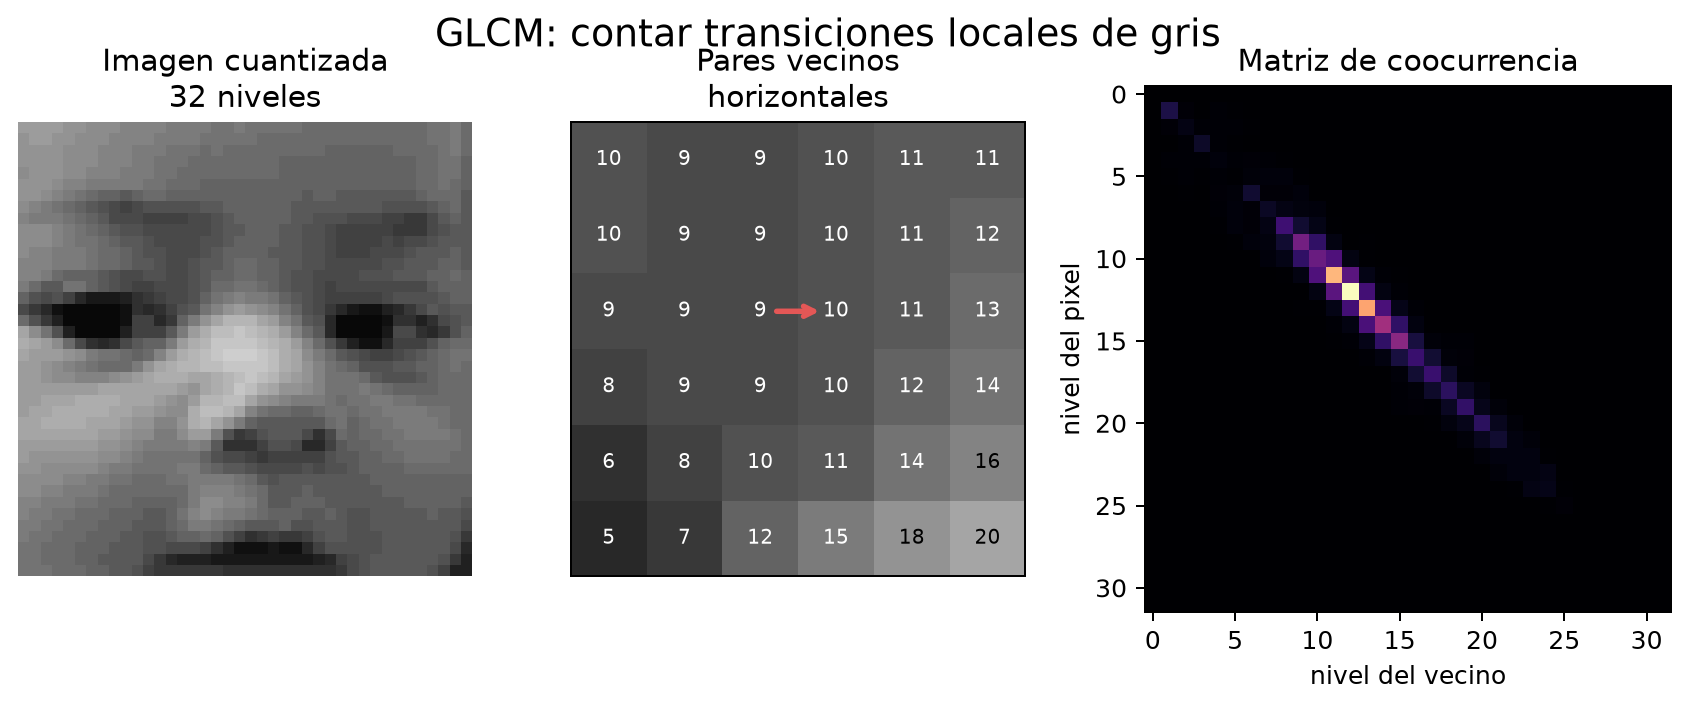
\includegraphics[width=0.95\linewidth]{texture_glcm.png}

    \vspace{0.1cm}
    \small
    Una GLCM es una matriz donde la entrada $(i,j)$ guarda con qué frecuencia un píxel de nivel de gris $i$ aparece junto a un vecino de nivel $j$. De cada GLCM extraemos seis números: contraste, disimilitud, homogeneidad, uniformidad, energía y correlación.
\end{frame}

\begin{frame}{Features: Textura -- bordes y entropía}
    \centering
    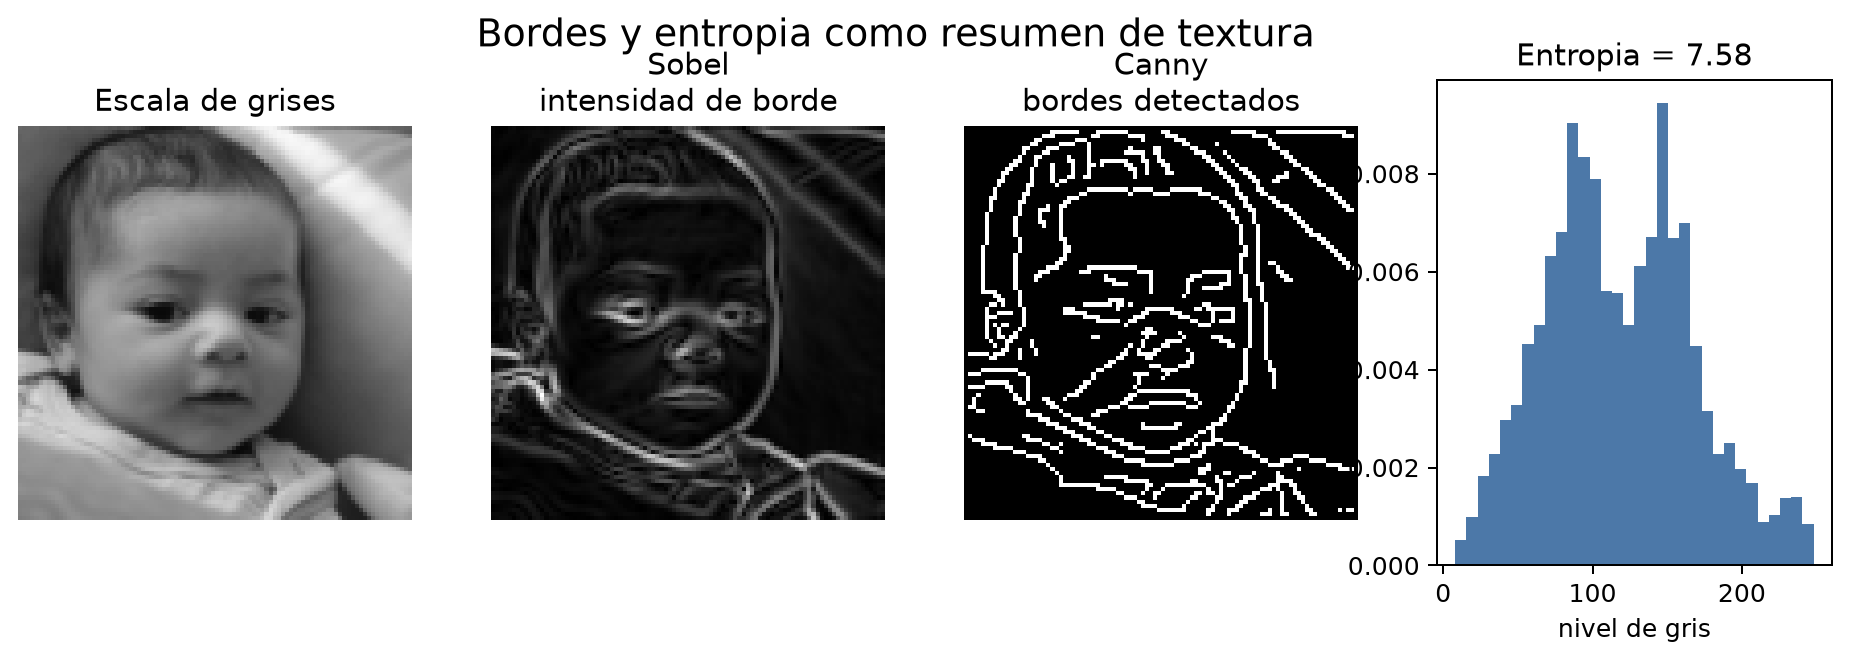
\includegraphics[width=0.95\linewidth]{texture_edges_entropy.png}

    \vspace{0.1cm}
    \small
    Sobel resume la intensidad de los bordes, Canny cuenta píxeles marcados como borde, y la entropía mide qué tan distribuido está el histograma de intensidades.
\end{frame}

\begin{frame}{Features: Gradientes HOG}
    El algoritmo HOG (Histograma de Gradientes Orientados) se enfoca puramente en las formas globales y las direcciones de los contornos.

    \begin{itemize}
        \item Divide la imagen en celdas compactas de $8 \times 8$ píxeles.
        \item En cada celda, calcula la dirección del gradiente del brillo.
        \item Agrupa esas direcciones en un histograma de 9 orientaciones (de $0^\circ$ a $180^\circ$).
    \end{itemize}
\end{frame}

\begin{frame}{Features: Frecuencia}
    Una imagen en escala de grises puede verse como una señal 2D.
    \begin{itemize}
        \item Frecuencias bajas: cambios suaves de iluminación y forma general.
        \item Frecuencias altas: bordes finos, ruido y textura pequeña.
    \end{itemize}

    Restamos la media de la imagen y aplicamos la Transformada de Fourier 2D:
    \[
        F(u,v)=\sum_x\sum_y I_c(x,y)e^{-2\pi i(ux/H+vy/W)}
    \]

    Usamos la magnitud del espectro:
    \[
        M(u,v)=\log(1+|F(u,v)|)
    \]
\end{frame}

\begin{frame}{Features: Frecuencia -- FFT 2D}
    \centering
    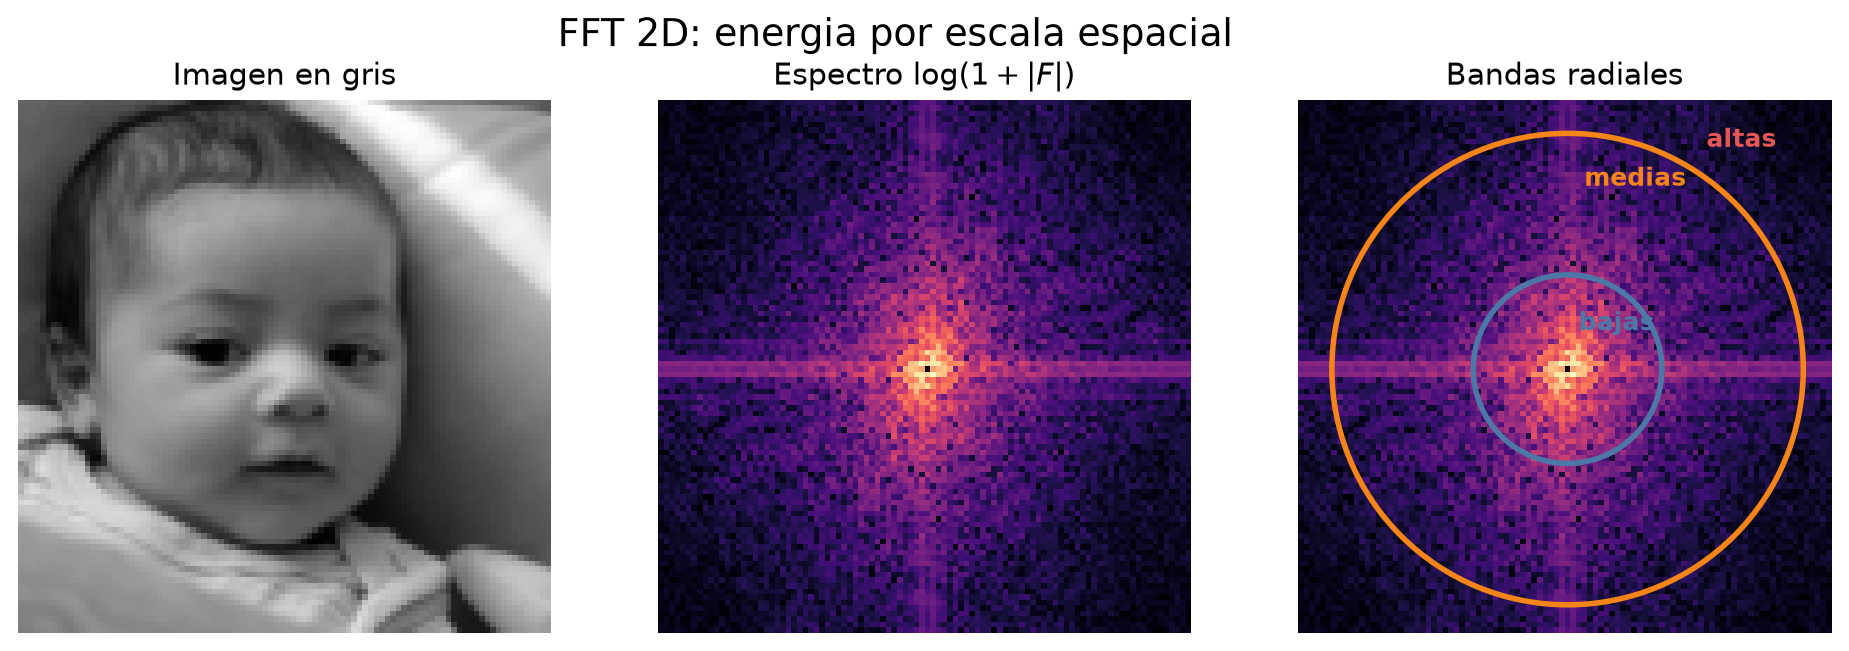
\includegraphics[width=0.95\linewidth]{frequency_fft_spectrum.png}

    \vspace{0.1cm}
    \small
    Después de centrar el espectro, el centro representa variaciones suaves y las zonas alejadas del centro representan cambios más rápidos.
\end{frame}

\begin{frame}{Features: Frecuencia -- perfil radial}
    \centering
    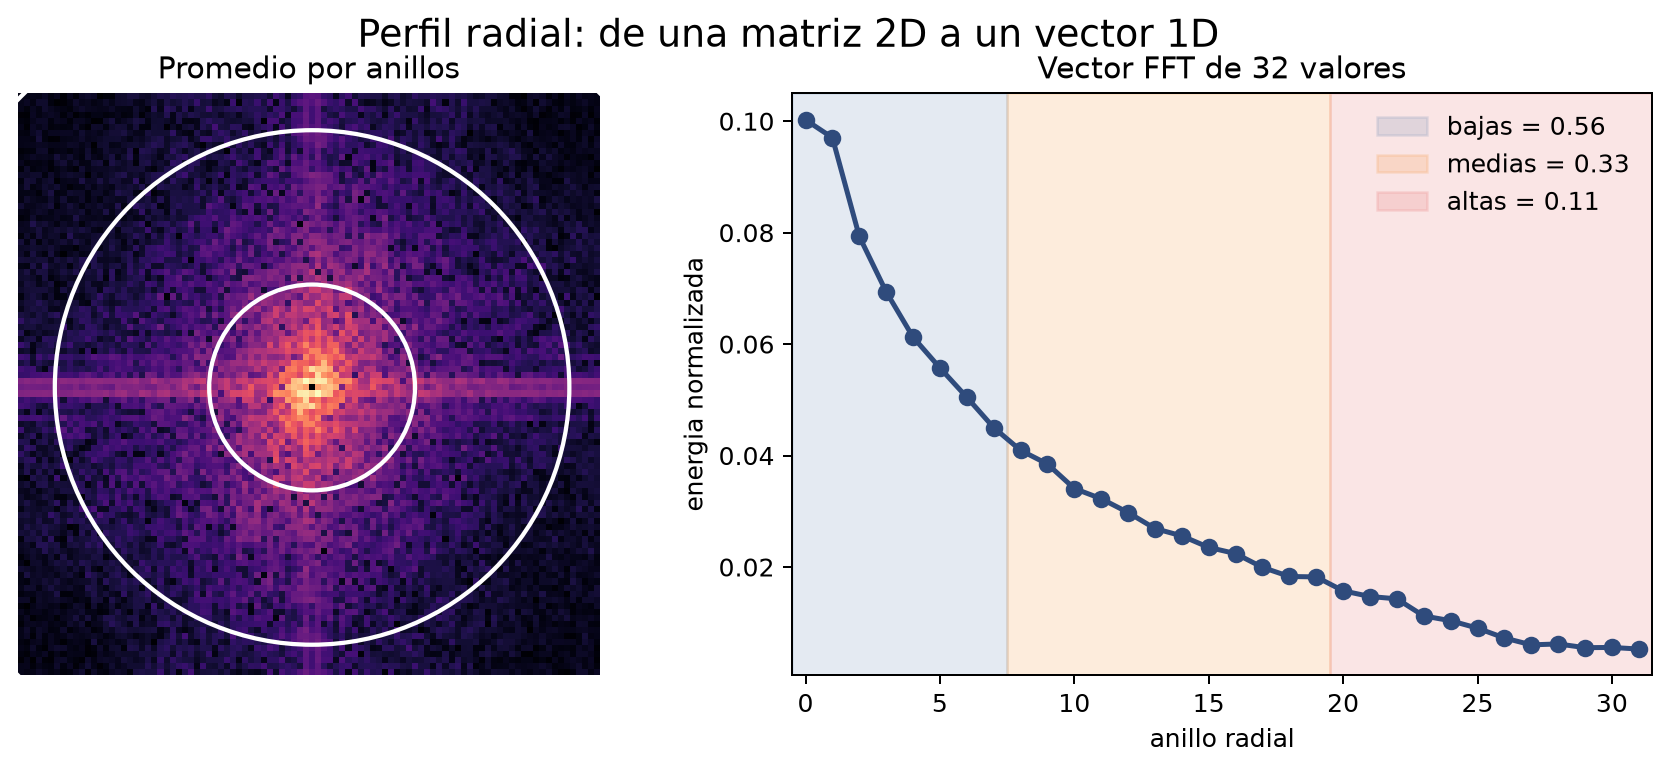
\includegraphics[width=0.74\linewidth]{frequency_radial_profile.png}

    \vspace{0.05cm}
    \scriptsize
    Promediamos $M(u,v)$ en 32 anillos concéntricos para convertir el espectro 2D en un vector:
    \[
        p_k=\frac{1}{|A_k|}\sum_{(u,v)\in A_k} M(u,v)
    \]
    \[
        \mathrm{baja}=\sum_{k=0}^{7}p_k,\quad
        \mathrm{media}=\sum_{k=8}^{19}p_k,\quad
        \mathrm{alta}=\sum_{k=20}^{31}p_k
    \]
    También guardamos las relaciones $\mathrm{alta}/\mathrm{baja}$ y $\mathrm{media}/\mathrm{baja}$.
\end{frame}

\begin{frame}{Features: Frecuencia -- DCT}
    \centering
    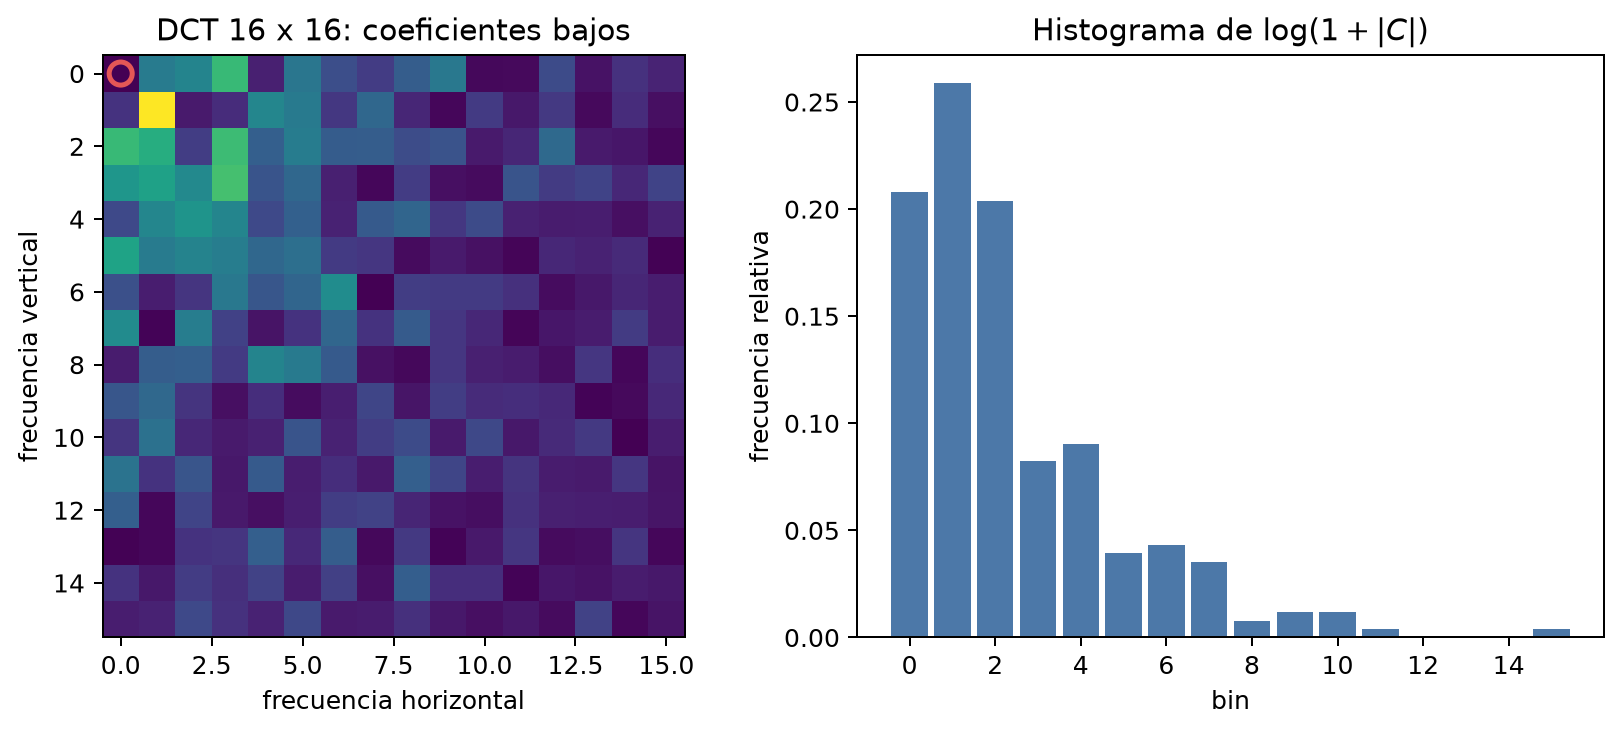
\includegraphics[width=0.82\linewidth]{frequency_dct.png}

    \vspace{0.05cm}
    \small
    La DCT también representa la imagen como suma de patrones de frecuencia, pero usando cosenos. Tomamos el bloque $16 \times 16$, quitamos el coeficiente constante y armamos un histograma de $\log(1+|C|)$ con 16 bins.

    \[
        32\ \text{perfil radial} + 5\ \text{bandas y ratios} + 16\ \text{DCT} = 53
    \]
\end{frame}

\begin{frame}{Features: Píxeles}
    Usar directamente los píxeles como features.\\
    \begin{itemize}
        \item Se achica primero la imagen a $32 \times 32$.
        \item Es lo más simple.
        \item Se puede usar escala de grises o los canales RGB.
    \end{itemize}
\end{frame}

\begin{frame}{Los modelos}
\begin{table}[]
    \centering
    \begin{tabular}{c|c}
        Modelo & Features\\ \hline
        Naive Bayes & Píxeles grises $32 \times 32$ \\
        Regresión logística & Color+píxeles grises con PCA \\
        SVM lineal & Todas las features \\
        Árbol de decisión & Color+textura+frecuencia\\
        Random Forest & Color+textura+frecuencia\\
        Gradient Boosting & Color+textura+frecuencia\\
        k-NN & Píxeles grises con PCA\\
        LDA & Todas las features con PCA\\
        QDA & Todas las features con PCA\\
        SVM con kernel RBF & Todas las features con PCA\\
        Red neuronal & Todas las features con PCA\\
    \end{tabular}
    \caption{Modelos y features probados}
    \label{tab:placeholder}
\end{table}
\end{frame}

\begin{frame}{El enfoque ganador: diferencias locales de píxeles}
    La idea es analizar los patrones finos en las texturas de la piel.\\
    Empezamos pasando las imágenes a blanco y negro y calculando la matriz de diferencias entre píxeles vecinos.
    
\includegraphics[scale=0.35]{09_diferencias_locales.png}
\end{frame}

\begin{frame}
    Cuantizamos los valores  en un rango de 0 a 8 y dividimos las matrices en $16$ celdas
    \includegraphics[scale=0.7]{clipped_difference.png}
\end{frame}

\begin{frame}
\begin{itemize}
    \item Sobre cada una de estas celdas obtenemos la matriz de coocurrencias entre parejas de píxeles.
    \item Para cada pareja de píxeles, se cuenta cuántas veces ocurre en cada celda.
    \item Esto resulta en $7 \times 16 \times 81 = 9072$ features.
    \item Finalmente se aplica PCA y whitening, reduciendo el número de features a 128.
\end{itemize}
Con esto se entrena un clasificador SVM con kernel RBF y regularización $C = 3.0$
\end{frame}


\begin{frame}{Resultados}
    \centering 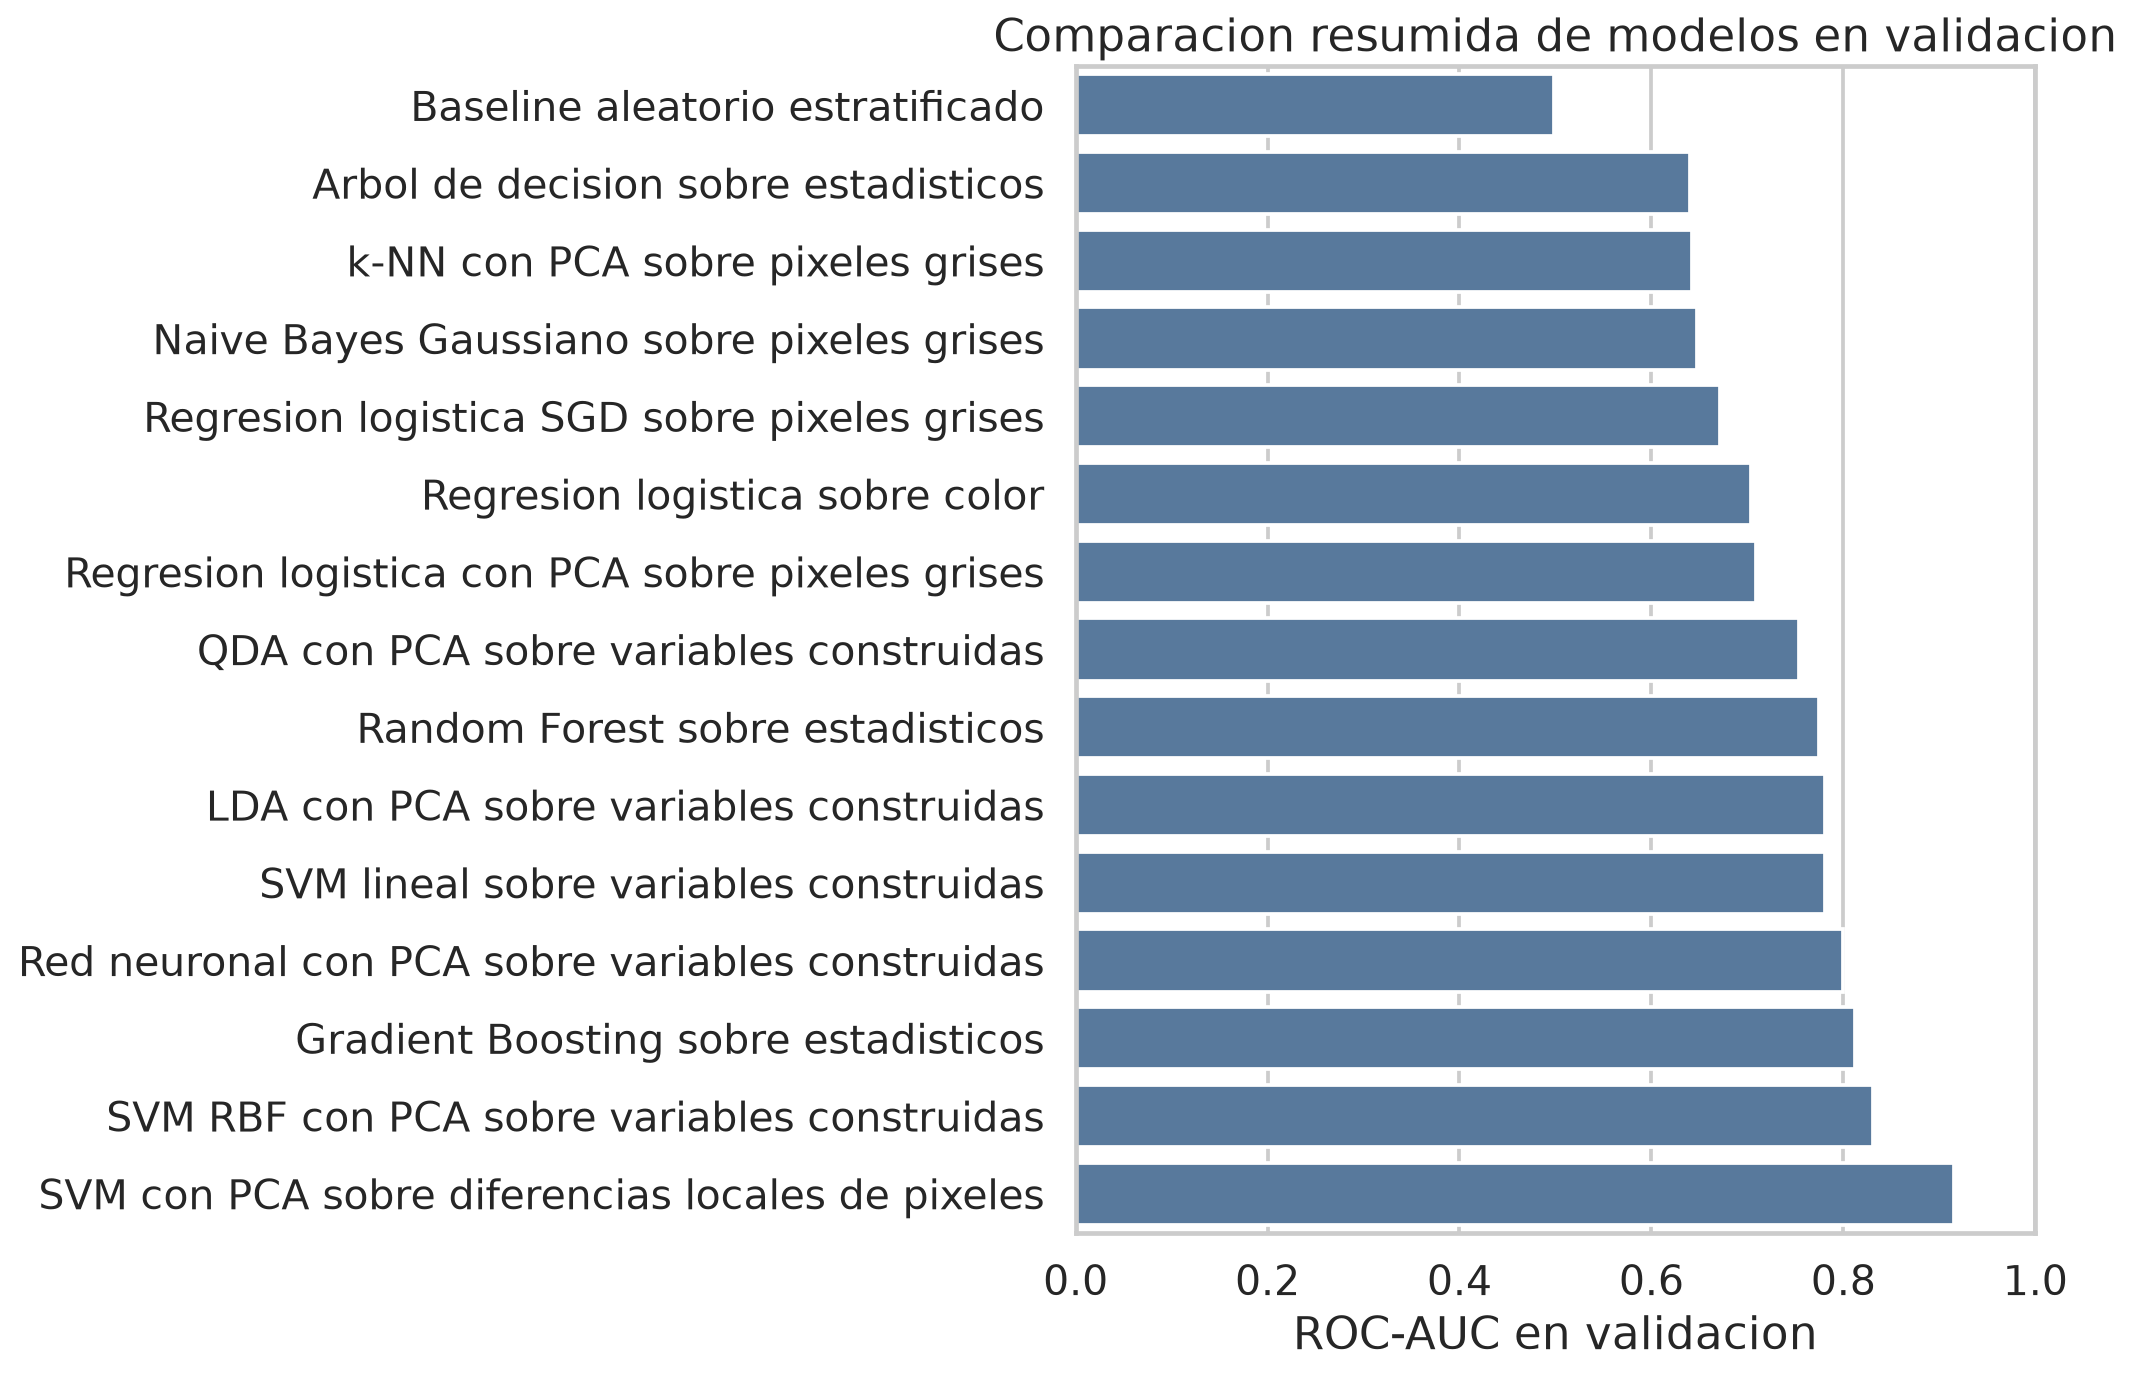
\includegraphics[width=\linewidth]{reports/figures/12_validacion_roc_auc_modelos_resumida.png}
\end{frame}

\begin{frame}
    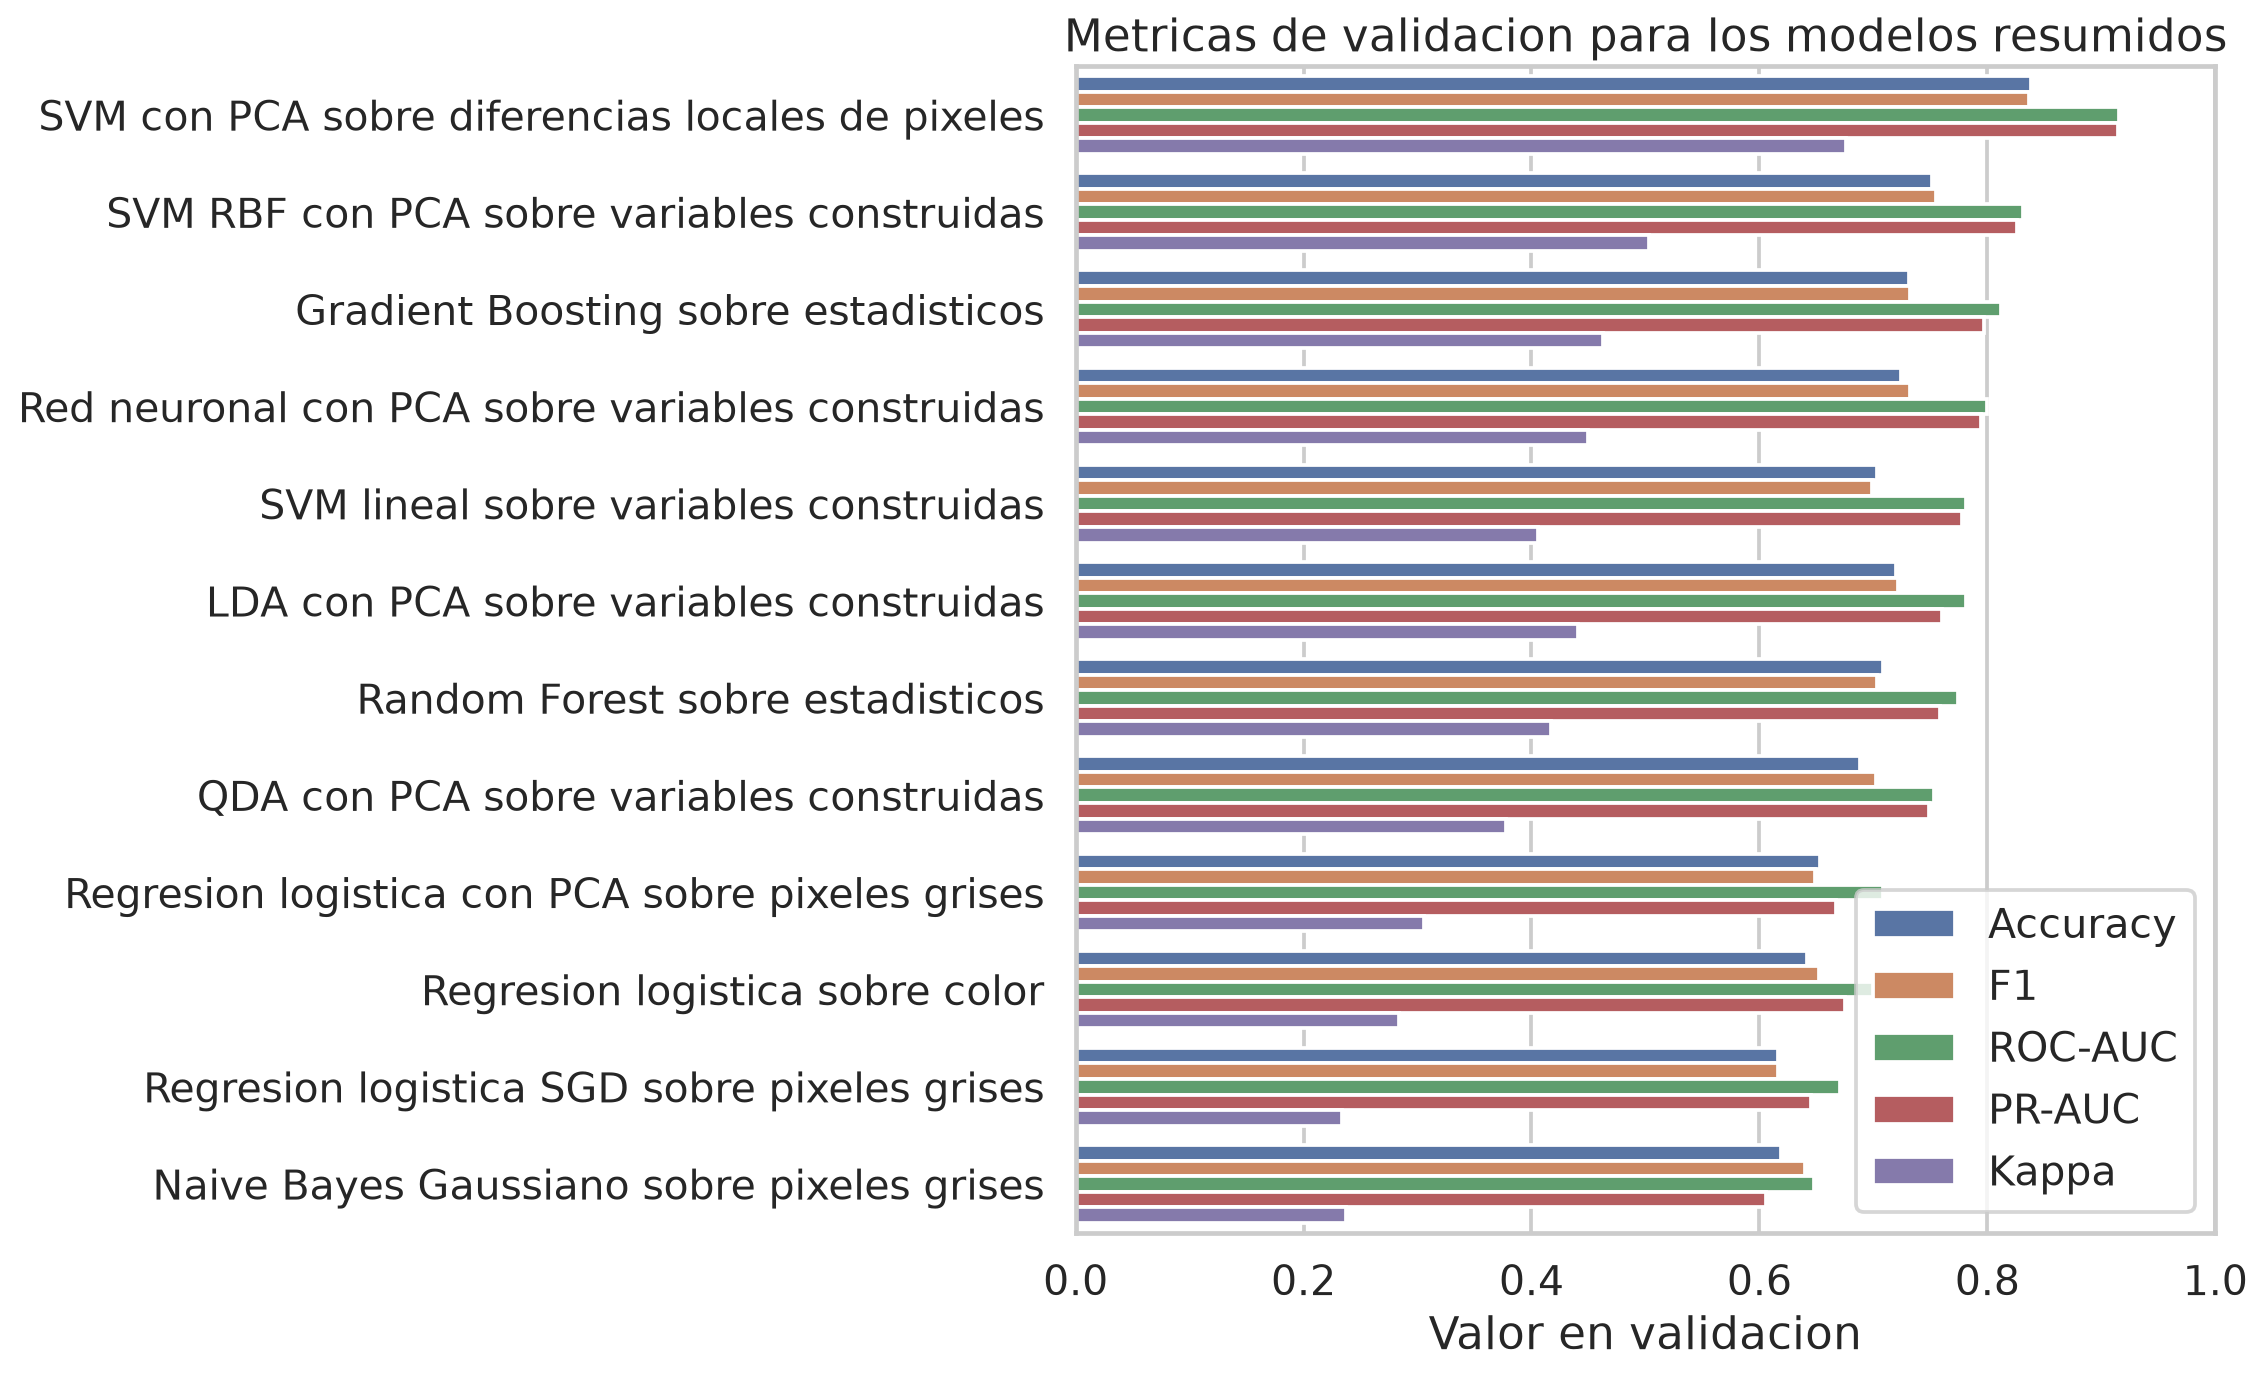
\includegraphics[width=\linewidth]{reports/figures/13_validacion_metricas_modelos_resumida.png}
\end{frame}

\begin{frame}
    
\includegraphics[scale=0.37]{04_metricas_test.png}
\end{frame}

\begin{frame}
    
\includegraphics[scale=0.65]{05_matriz_confusion.png}
\end{frame}

\begin{frame}
    
\includegraphics[scale=0.45]{07_scores_por_clase.png}
\end{frame}

\begin{frame}
    
\includegraphics[scale=0.37]{06_curvas_roc_pr.png}
\end{frame}

\begin{frame}{Conclusiones}
\begin{itemize}
    \item Es posible distinguir caras reales de las generadas por StyleGAN3 con buen rendimiento: el mejor modelo alcanza $\approx 82\%$ de accuracy y ROC-AUC $\approx 0.90$ en test.
    \item El enfoque de diferencias locales de píxeles (coocurrencias de residuos $+$ PCA/whitening $+$ SVM RBF) superó a todas las features clásicas, con unos $8$ puntos más de accuracy y de ROC-AUC que el mejor modelo sobre variables construidas.
    \item La señal que delata a las imágenes generadas está en las texturas finas, no en el contenido semántico (color o formas globales): el generador deja huellas a nivel de píxel.
    \item Los errores se reparten de forma pareja entre ambas clases ($261$ vs.\ $277$), sin sesgo hacia reales o generadas.
    \item \textbf{Trabajo futuro:} evaluar la generalización a otros generadores (otras GANs, modelos de difusión) y la robustez frente a compresión y reescalado.
\end{itemize}
\end{frame}

\end{document}
